\usetikzlibrary{arrows.meta,calc,decorations.pathreplacing,fit}

\tikzset{
    simple wire/.style={very thick,>=Latex},
    wire/.style={line width=1.5pt,>=Latex},
    wire small/.style={line width=1pt,>=Latex},
    binLabel/.style={font=\tt},
    hiBox/.style={red, very thick, draw},
    >=Latex,
}
\begin{frame}[fragile,label=opcodeHW]{extracting bits in hardware}
    % FIXME: diagram: wire bundle splitting getting opcode
    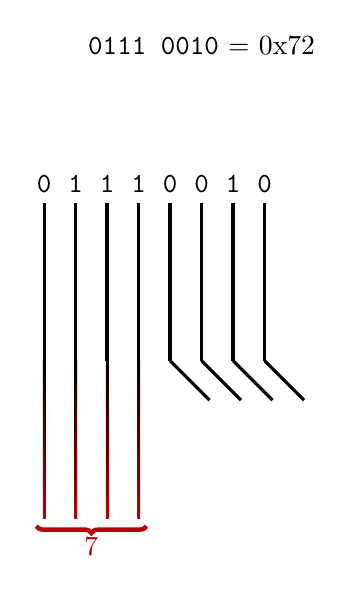
\begin{tikzpicture}
\foreach \x/\v in {0/0,0.4/1,0.8/1,1.2/1,1.6/0,2.0/0,2.4/1,2.8/0} {
    \draw[simple wire] (\x, 0) node[above] (\x-\v-num) {\tt\v} -- (\x, -2);
};
\foreach \x/\v in {0/0,0.4/0,0.8/1,1.2/0} {
    %\draw[simple wire,blue!70!black] (\x, -2) -- (\x, -4);
    \fill[top color=black,bottom color=red!70!black] ($(\x, -2) + (-.5pt, 0)$) rectangle ($(\x, -4) + (.5pt, 0)$);
};
\foreach \x/\v in {1.6/0,2.0/0,2.4/0,2.8/0} {
    \draw[simple wire] (\x, -2) -- ++(.5, -.5);
};
\node[anchor=center] at (2,2) {{\tt 0111 0010} = 0x\myemph{7}2};
        \node[fit={(0, -2) (1.6, -2)},red,ultra thick] {};

        \draw[red!70!black,ultra thick,decorate,decoration={brace,mirror}] (-.1, -4.1) -- (1.3, -4.1)
            node[midway,below] {7};
    \end{tikzpicture}
\end{frame}

